%%%%%%%%%%%%%%%%%%%%%%%%%%%%%%%%%%%%%%%%%
% Beamer Presentation
% LaTeX Template
% Version 1.0 (10/11/12)
%
% This template has been downloaded from:
% http://www.LaTeXTemplates.com
%
% License:
% CC BY-NC-SA 3.0 (http://creativecommons.org/licenses/by-nc-sa/3.0/)
%
%%%%%%%%%%%%%%%%%%%%%%%%%%%%%%%%%%%%%%%%%

%----------------------------------------------------------------------------------------
%   PACKAGES AND THEMES
%----------------------------------------------------------------------------------------

%\documentclass{beamer}
\documentclass[aspectratio=169]{beamer}
\mode<presentation> {

  % The Beamer class comes with a number of default slide themes
  % which change the colors and layouts of slides. Below this is a list
  % of all the themes, uncomment each in turn to see what they look like.

  %\usetheme{default}
  %\usetheme{AnnArbor}
  %\usetheme{Antibes}
  %\usetheme{Bergen}
  %\usetheme{Berkeley}
  %\usetheme{Berlin}
  %\usetheme{Boadilla}
  %\usetheme{CambridgeUS}
  %\usetheme{Copenhagen}
  %\usetheme{Darmstadt}
  %\usetheme{Dresden}
  %\usetheme{Frankfurt}
  %\usetheme{Goettingen}
  %\usetheme{Hannover}
  %\usetheme{Ilmenau}
  %\usetheme{JuanLesPins}
  %\usetheme{Luebeck}
  \usetheme{Madrid}
  %\usetheme{Malmoe}
  %\usetheme{Marburg}
  %\usetheme{Montpellier}
  %\usetheme{PaloAlto}
  %\usetheme{Pittsburgh}
  %\usetheme{Rochester}
  %\usetheme{Singapore}
  %\usetheme{Szeged}
  %\usetheme{Warsaw}

  % As well as themes, the Beamer class has a number of color themes
  % for any slide theme. Uncomment each of these in turn to see how it
  % changes the colors of your current slide theme.

  %\usecolortheme{albatross}
  %\usecolortheme{beaver}
  %\usecolortheme{beetle}
  %\usecolortheme{crane}
  %\usecolortheme{dolphin}
  %\usecolortheme{dove}
  %\usecolortheme{fly}
  %\usecolortheme{lily}
  %\usecolortheme{orchid}
  %\usecolortheme{rose}
  %\usecolortheme{seagull}
  %\usecolortheme{seahorse}
  \usecolortheme{whale}
  %\usecolortheme{wolverine}

  %\setbeamertemplate{footline} % To remove the footer line in all slides uncomment this line
  %\setbeamertemplate{footline}[page number] % To replace the footer line in all slides with a simple slide count uncomment this line

  %\setbeamertemplate{navigation symbols}{} % To remove the navigation symbols from the bottom of all slides uncomment this line
}
\usefonttheme[onlymath]{serif}
%\usepackage{epsfig}
\usepackage{graphicx} % Allows including images
\usepackage{booktabs} % Allows the use of \toprule, \midrule and \bottomrule in tables
\usepackage{multimedia} % 
%\usepackage{animate}
%\usepackage{tikz}
%\usepackage{lipsum}

\usepackage{tikz} 
\usetikzlibrary{tikzmark,overlay-beamer-styles,positioning,calc}
%\usetikzlibrary{tikzmark,
%\usetikzlibrary{tikzmark}
%\usetikzlibrary{arrows,shapes}
%\newcommand{\tikzmark}[1]{\tikz[remember picture] \node[coordinate] (#1) {#1};}
\newcommand{\be}{\begin{equation*}}
\newcommand{\ee}{\end{equation*}}
\newcommand{\ol}{\overline}
\newcommand{\p}{\partial}
\newcommand{\pdv}[2]{\frac{\partial \, #1}{\partial #2}}
\newcommand{\etal}{ {\it et al.} }
%----------------------------------------------------------------------------------------
%   TITLE PAGE
%----------------------------------------------------------------------------------------

\title[CHARTS]{Candidate CHARTS Model Summary} % The short title appears at the bottom of every slide, the full title is only on the title page

\author[]{Brad Johnson\\Liz Holzenthal\\Rusty Permenter \\Kevin Hodgens } % Your name
\institute[ERDC] % Your institution as it will appear on the bottom of every slide, may be shorthand to save space
{USACE Engineering Research and Devlelopment Center \\ % Your institution for the title page
\medskip
\textit{} % Your email address
}
%\date{\today} % Date, can be changed to a custom date
\date{\vspace*{-0cm}\\ Jan, 2025} % Date, can be changed to a custom date

\begin{document}

\begin{frame}
  %\titlepage % Print the title page as the first slide
  \begin{columns}[c] % The "c" option specifies centered vertical alignment while the "t" option is used for top vertical alignment
    
    \column{.3\textwidth} % Left column and width
    \titlepage % Print the title page as the first slide
%%     \vspace*{-1cm}
%%     \begin{center}
%% District PDT:\\
%% Kelly Legault (SAJ)\\
%% Gabriel Todaro (SAJ)
%%     \end{center}
    \column{.7\textwidth} % Right column and width
    \begin{figure}
            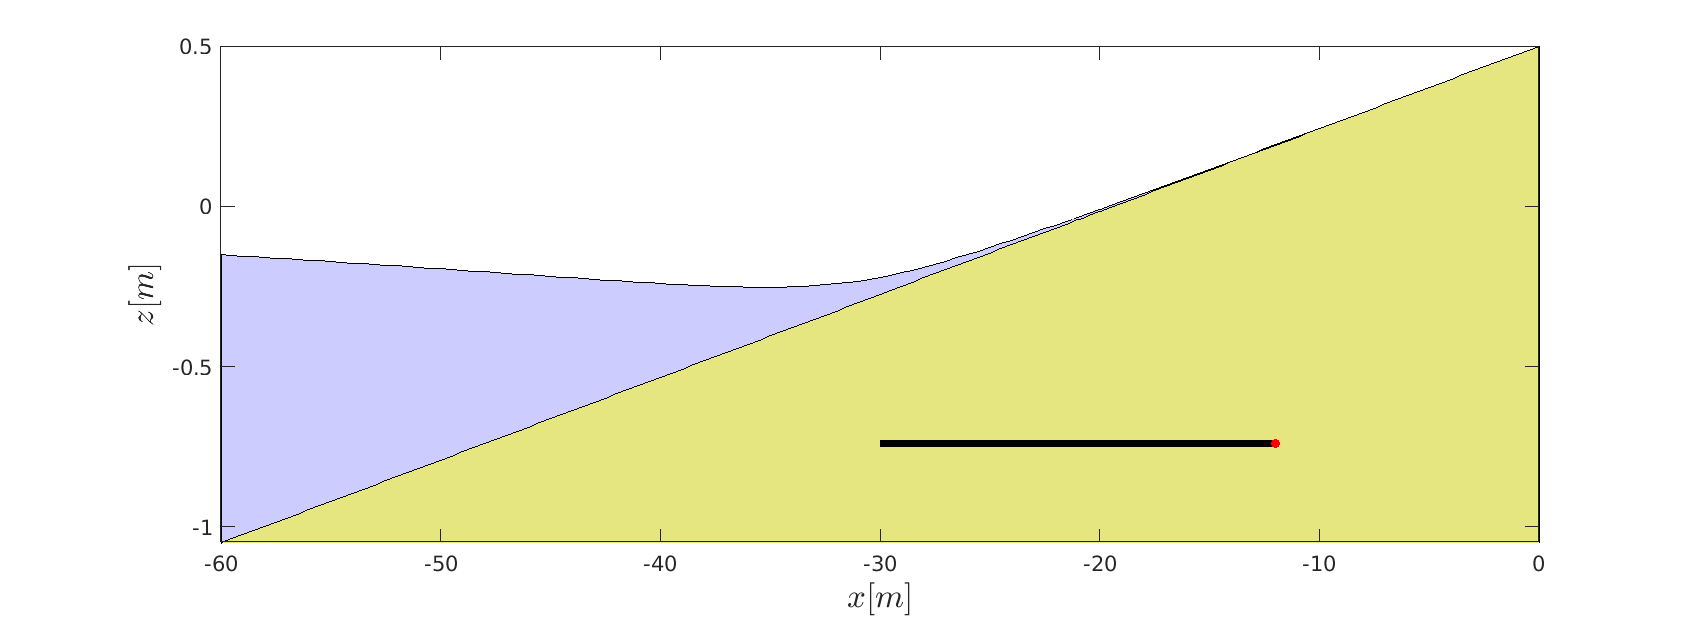
\includegraphics[width=1\linewidth]{./present.png}
      %\includegraphics[trim={0 1cm 0 0},clip,width=0.9\linewidth]{./breaking-wave-on-the-beach.jpg}
    \end{figure}
    
  \end{columns}
\end{frame}

%%%%%%%%%%%%%%%%%%%%%%%%%%%%%%%%%%%%%%%%%%%%%%%%%%%%%%%%%%%%%%%%%%%%%%%%%%%%%%%%%%%%%%%%%%%%%%%%%%%%

\begin{frame}
  \frametitle{Model Objectives}

  The CHART effort requires  simple, stable, and computationally efficient hydrodynamics framework that can be customized to meet USACE needs.
 \begin{columns}[c] % 
    
   \column{.9\textwidth} % Left column and width

  First incarnation hydro model:
 \begin{itemize}
 \item One-dimensional
 \item Phase-averaged but low-frequency resolving
 \item Based on NLSW
   \item includes forcing through boundaries, waves, winds ( but no wind generation) 
 \item Heuristic wet/dry
 \item Emphasis on simple and efficient
 \item Somewhat numerically diffusive (Fischer's) num soln, but steep slopes (or more accurately, large slope breaks) cause issues
 \item Includes numerical apparatus for two-scale closure approximations, including skewed wave-forms
 \end{itemize}
 \column{.1\textwidth} % Left column and width
 \end{columns}
 \end{frame}
%%%%%%%%%%%%%%%%%%%%%%%%%%%%%%%%%%%%%%%%%%%%%%%%%%%%%%%%%%%%%%%%%%%%%%%%%%%%%%%%%%%%%%%%%%%%%%%%%%%%
\begin{frame}
  \frametitle{Ponding}
  Overtopping capture, but no infiltration
    \centering
    \movie[externalviewer]{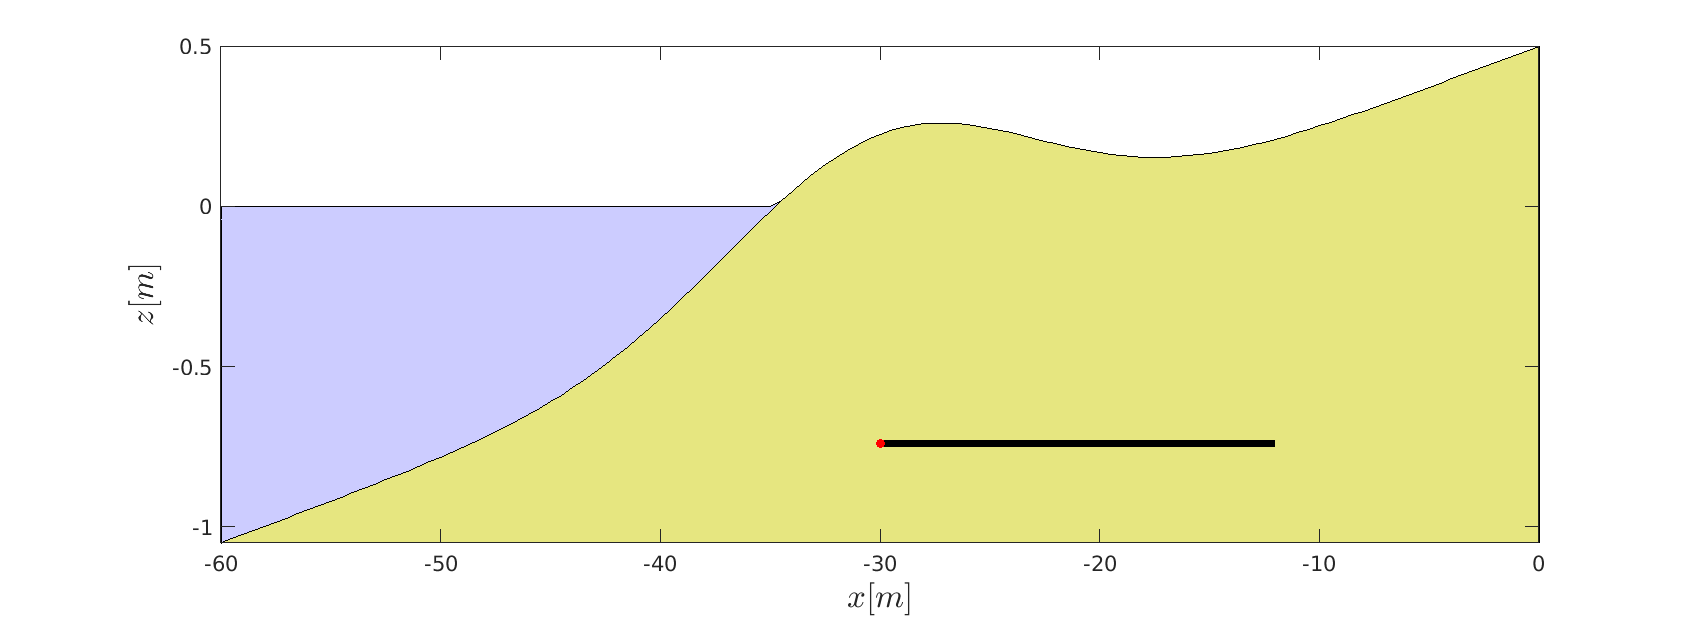
\includegraphics[width=\textwidth, keepaspectratio]{ponding.png}}{ponding.avi}
\end{frame}

%%%%%%%%%%%%%%%%%%%%%%%%%%%%%%%%%%%%%%%%%%%%%%%%%%%%%%%%%%%%%%%%%%%%%%%%%%%%%%%%%%%%%%%%%%%%%%%%%%%%
\begin{frame}
  \frametitle{Wave forcing}
  A one-line wave model:
  \begin{equation*}
    H_{i+1}=\min{\left(\left\{ H_i^2 \frac{c_i n_i}{c_{i+1} n_{i+1}}\right\}^{1/2},\gamma h_i\right)}
  \end{equation*}
  
    \centering
    \movie[externalviewer]{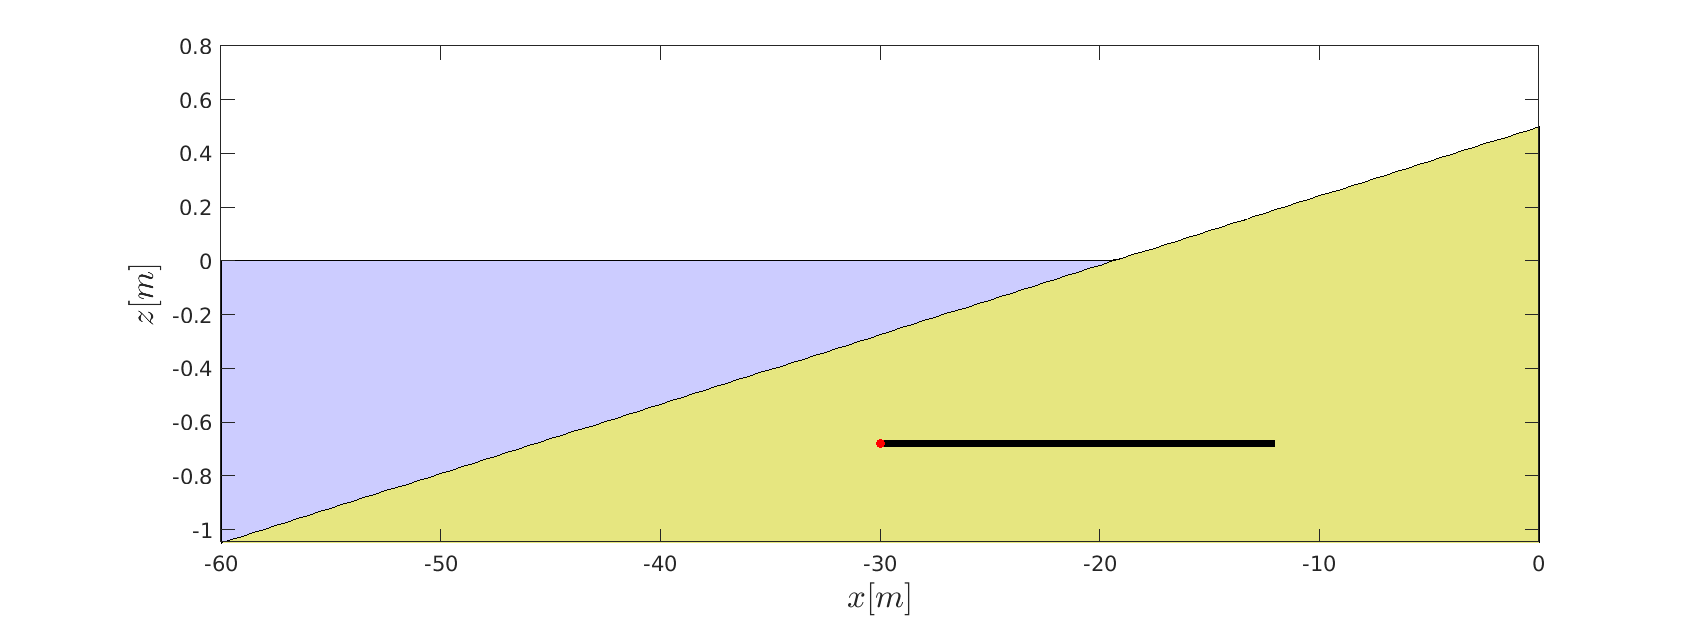
\includegraphics[width=\textwidth, keepaspectratio]{planarwithwaves.png}}{planarwithwaves.avi}
\end{frame}

%%%%%%%%%%%%%%%%%%%%%%%%%%%%%%%%%%%%%%%%%%%%%%%%%%%%%%%%%%%%%%%%%%%%%%%%%%%%%%%%%%%%%%%%%%%%%%%%%%%%
\begin{frame}
\frametitle{Equilibrium Transport Model}
A simple traction (or energetics) model that assumes transport is in equilib with forcing: 

\begin{equation*}
  \overline{q_{eq}} = \frac{8 B}{T} \sqrt{g (s-1) d_{50}^3}\int_0^T(\theta(t)-\theta_{cr})^{3/2} dt 
\end{equation*}

Bottom evolution is dictated by conservation of sand
\begin{equation*}
\pdv{z_b}{t} = -\frac{1}{1-n} \pdv{\overline{q_{eq}}}{x}
\end{equation*}
where $n$ is the bed porosity, which is solved numerically for the bed
evolution in time with an first-order time-explicit scheme with
second-order central differences in space.
\end{frame}
%%%%%%%%%%%%%%%%%%%%%%%%%%%%%%%%%%%%%%%%%%%%%%%%%%%%%%%%%%%%%%%%%%%%%%%%%%%%%%%%%%%%%%%%%%%%%%%%%%%%
\begin{frame}
  \frametitle{Equilibrium Transport Model With Waves} 
  \centering
  \movie[externalviewer]{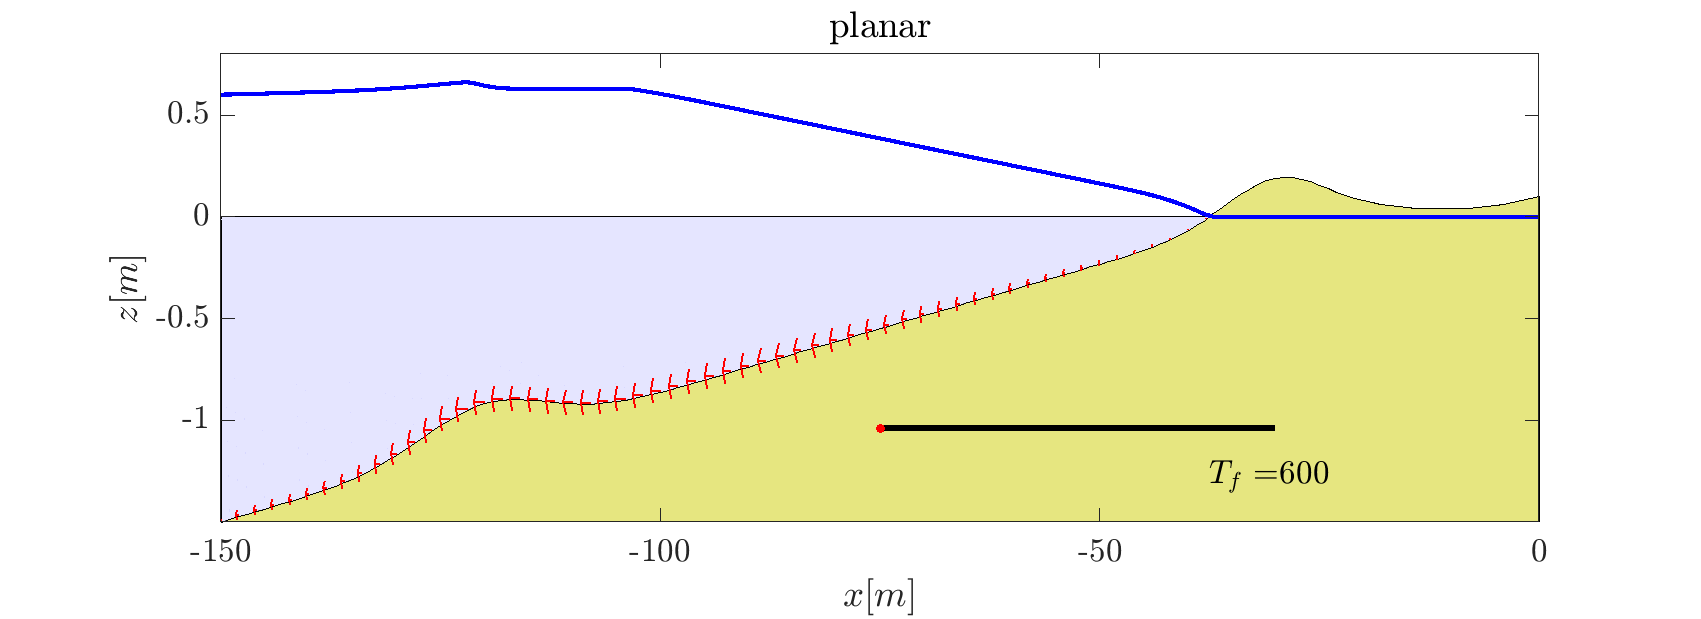
\includegraphics[width=\textwidth, keepaspectratio]
    {../../graphics/overwash_with_waves.png}}{../../graphics/overwash_with_waves.avi}
\end{frame}

%%%%%%%%%%%%%%%%%%%%%%%%%%%%%%%%%%%%%%%%%%%%%%%%%%%%%%%%%%%%%%%%%%%%%%%%%%%%%%%%%%%%%%%%%%%%%%%%%%%%
\begin{frame}
  \frametitle{Non-Equilibrium Transport Model} 

  Accounting for spatial gradients is achieved by equating gradients
  in transport $q$ and bed-pickup $P$ and fallout, $F$

  \begin{equation*}
    \pdv{\overline{q}}{x} = P-F 
  \end{equation*}
Fallout $F$ can be expressed in terms of near-bed concentration, $c$
as $F = w_f c = \frac{w_f}{u \delta} \overline{q} $ which makes use of
$q = u \delta c$ where $\delta$ is a bedload layer thickness $\sim 0.01m$.
Similarly, the pickup, $P = A \frac{w_f}{u \delta} \overline{q_{eq}}$
where $A$ is a modifier equal to 0 or 1 indicating the availability of sand in the bed
to be suspended.  Note that the formulation can also be represented with a disequilibrium model 
  \begin{equation*}
    \pdv{\overline{q}}{x} = \frac{A \overline{q_{eq}}  - \overline{q}}{L} \;\;\;\;\mbox{where}\;\;\; L = \frac{u \delta}{w_f}
  \end{equation*}
and $L$ has the physical interpretation of a horizontal advection
length that a particle travels while falling through the
boundary layer.
\end{frame}
%%%%%%%%%%%%%%%%%%%%%%%%%%%%%%%%%%%%%%%%%%%%%%%%%%%%%%%%%%%%%%%%%%%%%%%%%%%%%%%%%%%%%%%%%%%%%%%%%%%%
\begin{frame}
  \frametitle{Non-Equilibrium Transport Model} 
  \centering
  \movie[externalviewer]{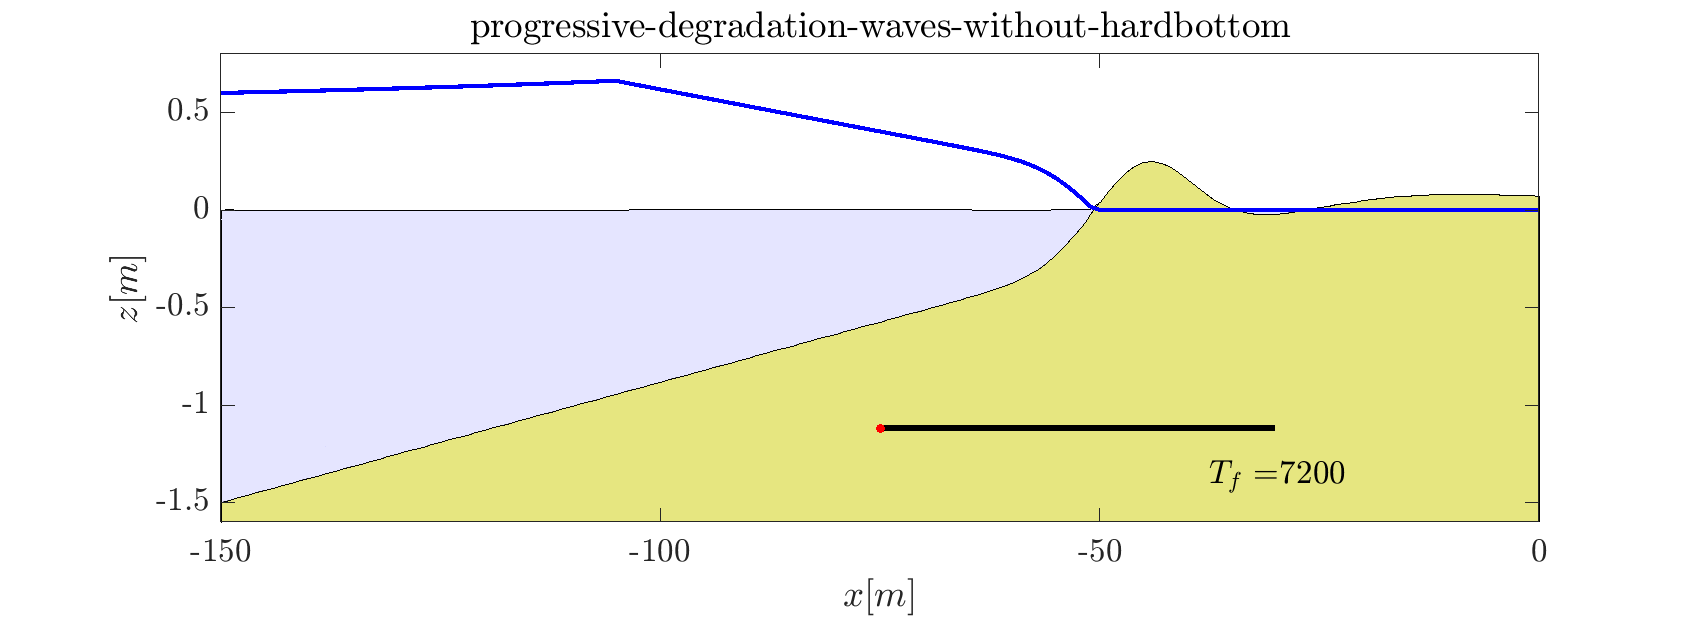
\includegraphics[width=\textwidth, keepaspectratio]
    {../../graphics/progressive_degradation_waves_without_hardbottom.png}}{../../graphics/progressive_degradation_waves_without_hardbottom.avi}
\end{frame}
%%%%%%%%%%%%%%%%%%%%%%%%%%%%%%%%%%%%%%%%%%%%%%%%%%%%%%%%%%%%%%%%%%%%%%%%%%%%%%%%%%%%%%%%%%%%%%%%%%%%
\begin{frame}
  \frametitle{Non-Equilibrium Transport Model} 
  \centering
  \movie[externalviewer]{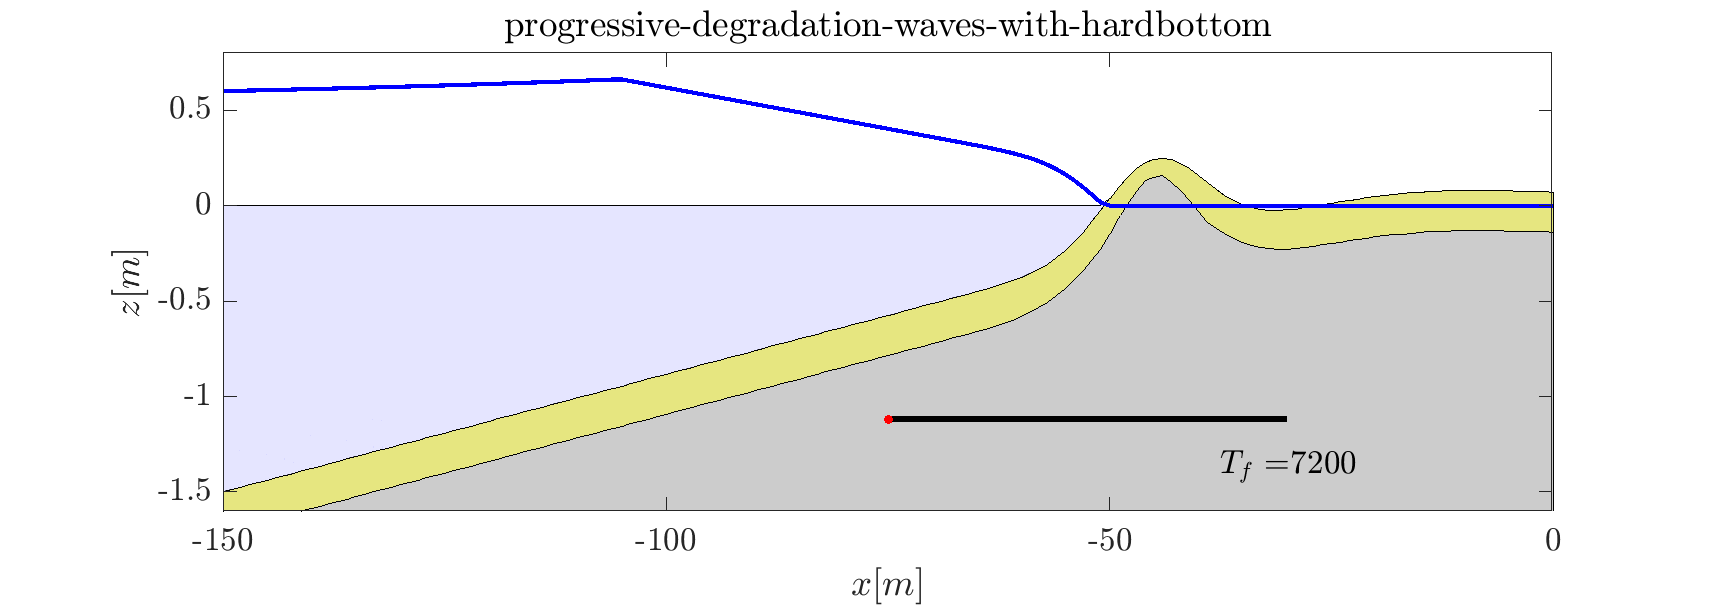
\includegraphics[width=\textwidth, keepaspectratio]
    {../../graphics/progressive_degradation_waves_with_hardbottom.png}}{../../graphics/progressive_degradation_waves_with_hardbottom.avi}
\end{frame}
%%%%%%%%%%%%%%%%%%%%%%%%%%%%%%%%%%%%%%%%%%%%%%%%%%%%%%%%%%%%%%%%%%%%%%%%%%%%%%%%%%%%%%%%%%%%%%%%%%%%
\begin{frame}
  \frametitle{Challenges}
  In cases of large slope ( esp with large concavity), MBC can cause instability  
  \centering
  \movie[externalviewer]{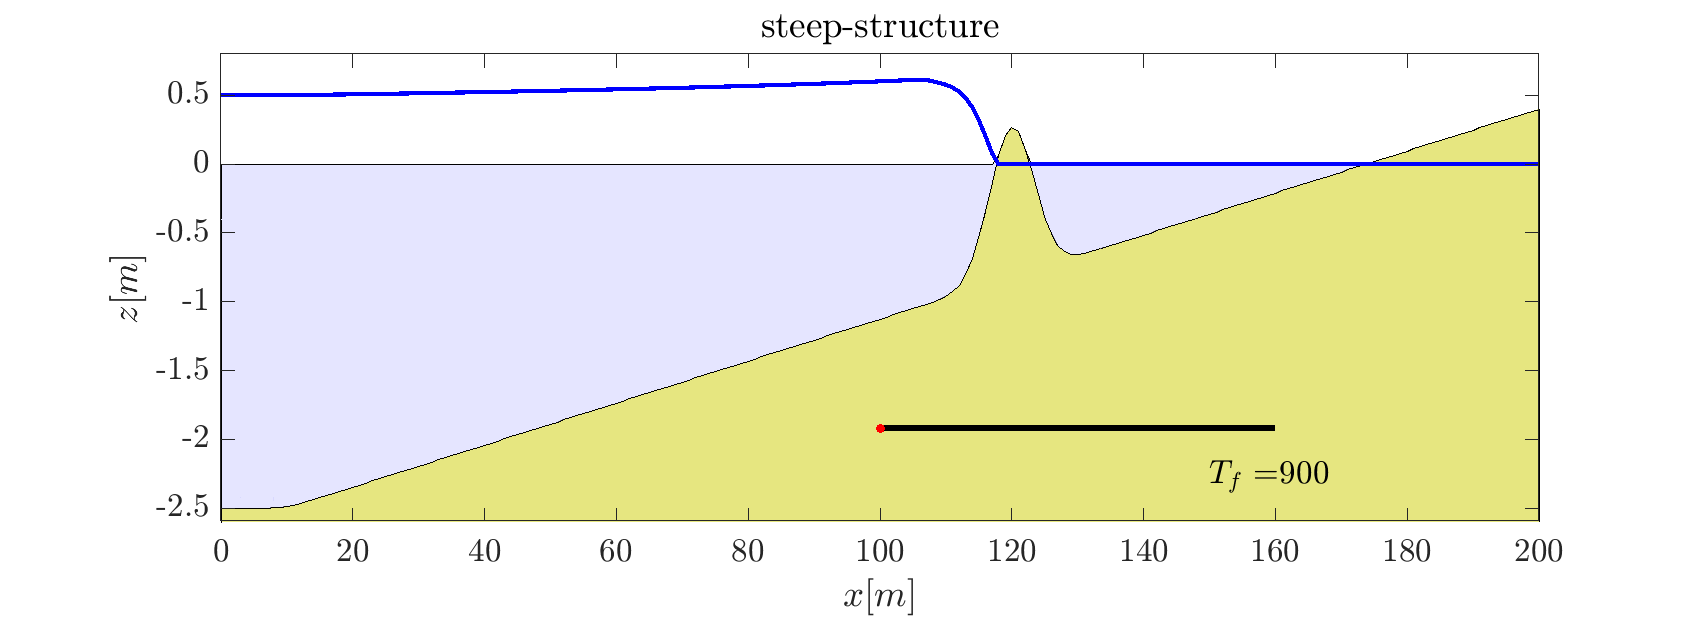
\includegraphics[width=\textwidth, keepaspectratio]
    {./steep_structure.png}}{./steep_structure.avi}
\end{frame}
%%%%%%%%%%%%%%%%%%%%%%%%%%%%%%%%%%%%%%%%%%%%%%%%%%%%%%%%%%%%%%%%%%%%%%%%%%%%%%%%%%%%%%%%%%%%%%%%%%%%
\begin{frame}
  \frametitle{Challenges} 
  Clock time for simulating 24 hrs 
  \begin{center}
    \begin{tabular}{ |c|c|c| } 
      \hline
      $H$ & 50$s$ \\ 
      \hline
      $H+W$ & 200$s$ \\
      \hline
      $H+S_{eq}$ & 60$s$  \\
      \hline
      $H+S_{neq}$ & 440$s$  \\ 
      \hline
    \end{tabular}
  \end{center}
  So these runtimes are getting close to being prohibitively large if we run 100K runs: 500 days on singe thread for non-equilibrium transport. 
\end{frame}
%%%%%%%%%%%%%%%%%%%%%%%%%%%%%%%%%%%%%%%%%%%%%%%%%%%%%%%%%%%%%%%%%%%%%%%%%%%%%%%%%%%%%%%%%%%%%%%%%%%%
\begin{frame}
  \frametitle{Next Steps and Considerations} 
  \begin{itemize}
  \item Runtimes can be improved, but improved by 25\%, not 75\%
  \item Improved MSBC is needed but tricky -- could add prohibitive numerical cost
  \item Ugly $2 \Delta x$ in hydro is difficult to remove from current
    field, but it's straightforward to remove it before doing the sed
    computations
  \item Still have option to shelve this work return to the old CSHORE/SBEACH workflow development
  \end{itemize}


\end{frame}

%%%%%%%%%%%%%%%%%%%%%%%%%%%%%%%%%%%%%%%%%%%%%%%%%%%%%%%%%%%%%%%%%%%%%%%%%%%%%%%%%%%%%%%%%%%%%%%%%%%%
  
\end{document}
